\section{Switches}
\label{switches}

\bigskip
The simplest kind of switch is an ``on-off'' switch, which either makes or breaks a connection. We often represent it with a symbol that looks like an old-fashioned knife switch, regardless of the switch's actual physical shape.  Special symbols do exist for some specific forms like slide switches or rocker switches, but those symbols aren't always used.\footnote{In fact, a quick web search reveals literally hundreds of different symbols that are claimed to represent various esoteric specialty switches, though it's dubious whether many of those symbols would be identifiable by anyone beyond the person who created them.}
\begin{center}
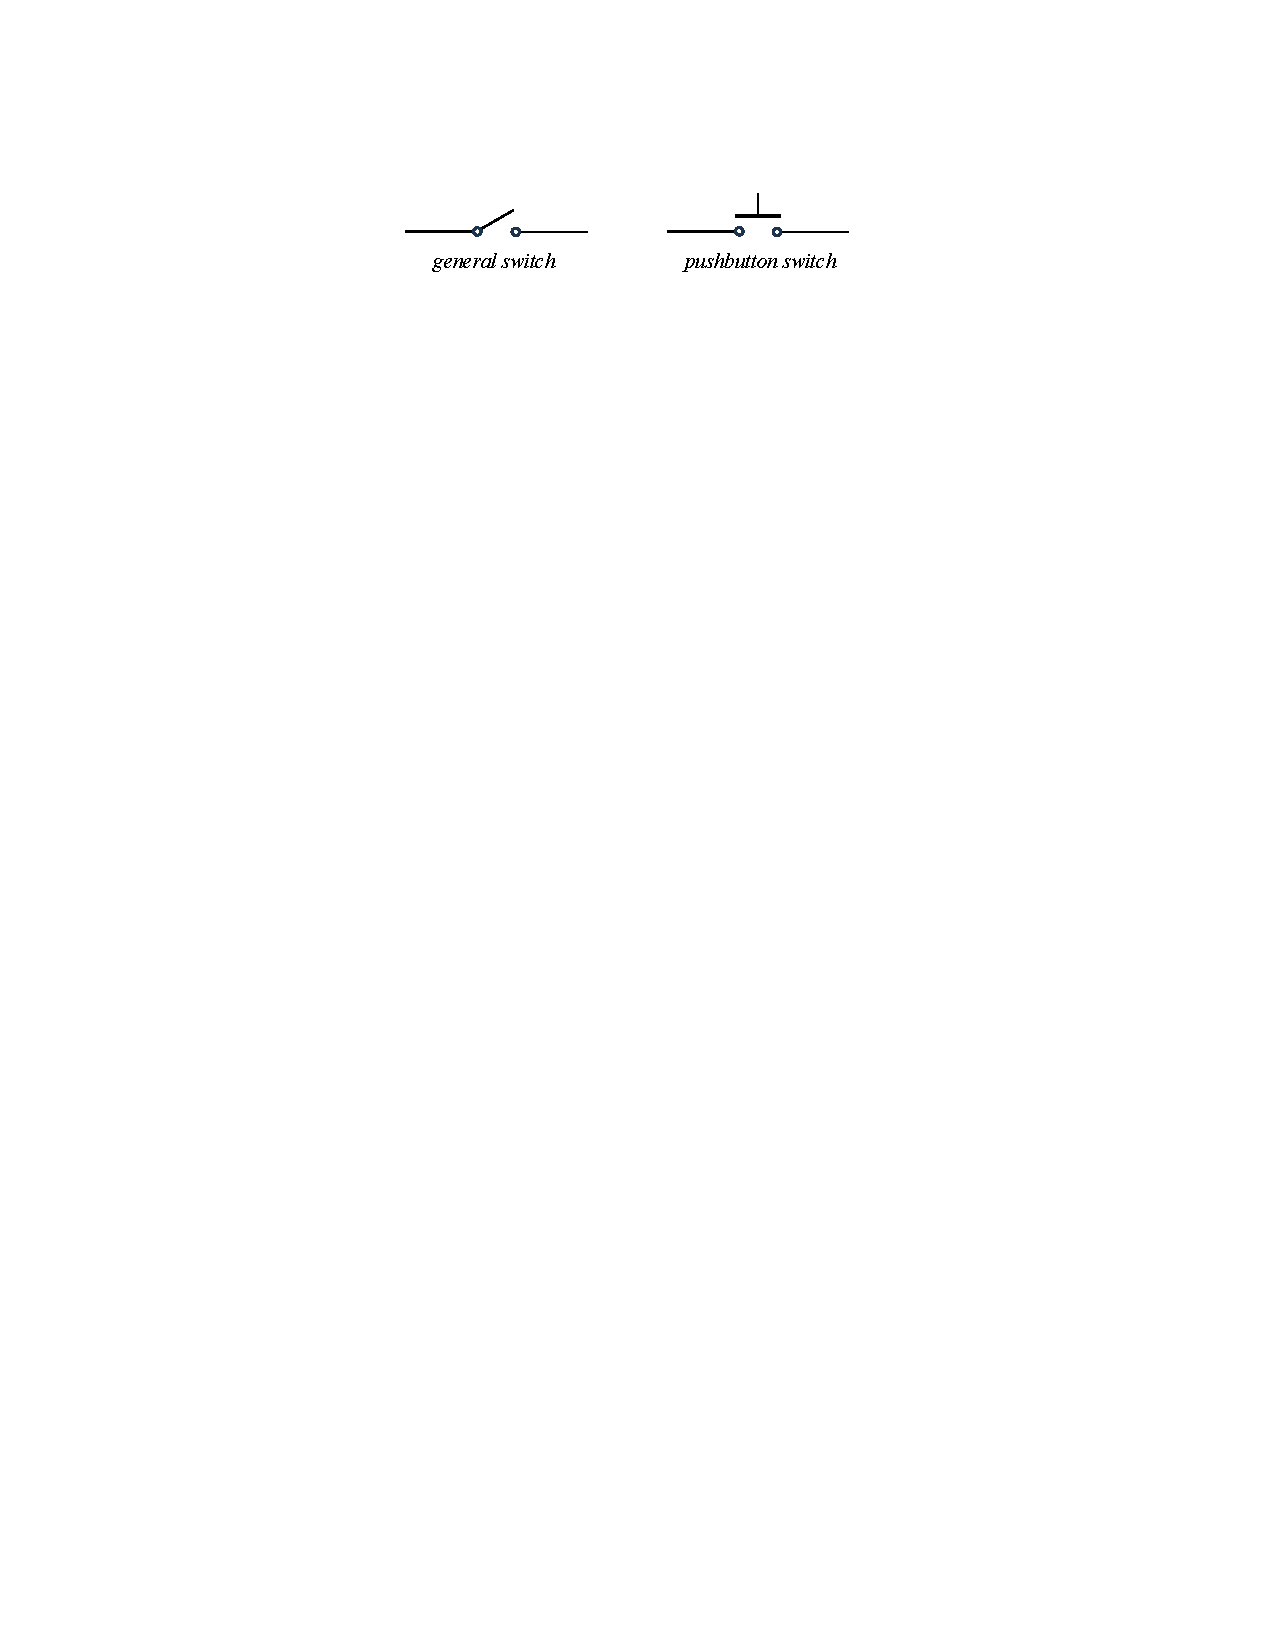
\includegraphics{appendices/switches/general_switch.pdf}
\end{center}
Another common type of switch has three-terminals, allowing a \textit{common} terminal to connect to either of two different outputs.  This is called a \textit{Single Pole Double Throw} (SPDT) switch, where each \textit{throw} is one of the two possible output connections.
The \textit{poles} in a switch are the number of separate circuits that are controlled by the switch's movement, as in the Double Pole Single Throw (DPST) and Double Pole Double Throw (DPDT) switches below.  The dotted line indicates that the two arms move together with a single flip of the switch.  By this naming convention, our humble on-off switch is an SPST.  One can also have triple poles and/or triple throws, written 3PDT or 3P3T; beyond that you often simply see an M for multiple, as in MPMT.
\begin{center}
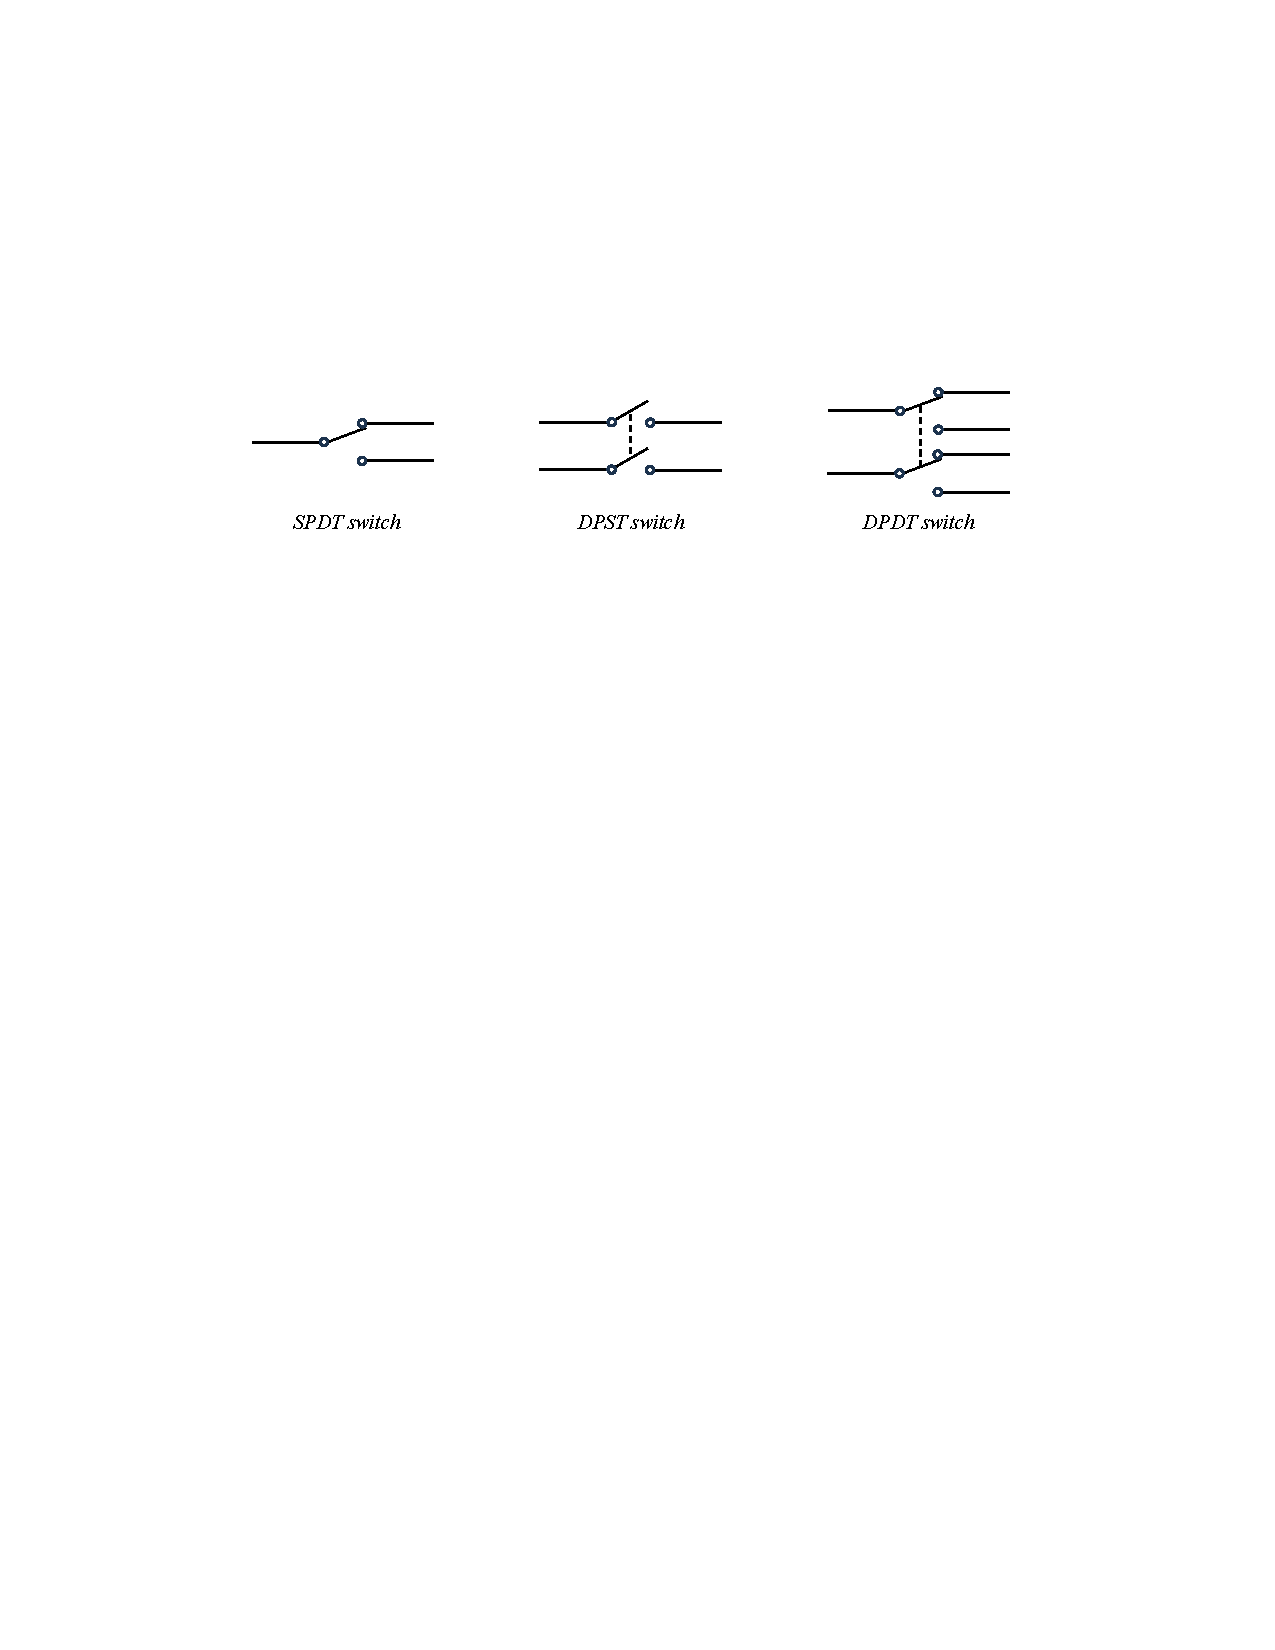
\includegraphics{appendices/switches/poles_and_throws.pdf}
\end{center}
One familiar application for SPDT switches is to control a  set of lights using two different switches, for instance at the top and bottom of a staircase. In the first diagram below, the light is connected when both switches are up or both switches are down.  In this context, builders and electricians call the SPDT switch a ``3-way switch,'' at least in the US and Canada.%
\footnote{In the UK and Australia, our 3-way switch is called a ``2-way switch,'' and our 4-way switch is called an ``intermediate switch,'' none of which is confusing at all.} When switches are needed in three or more locations, as in a large room with multiple doors, one or more ``4-way'' switches can be inserted. In the lower diagram below, the 4-way switch connects the two sides either straight through (red-to-red and black-to-black), or crossed, as they are drawn here.
\begin{center}
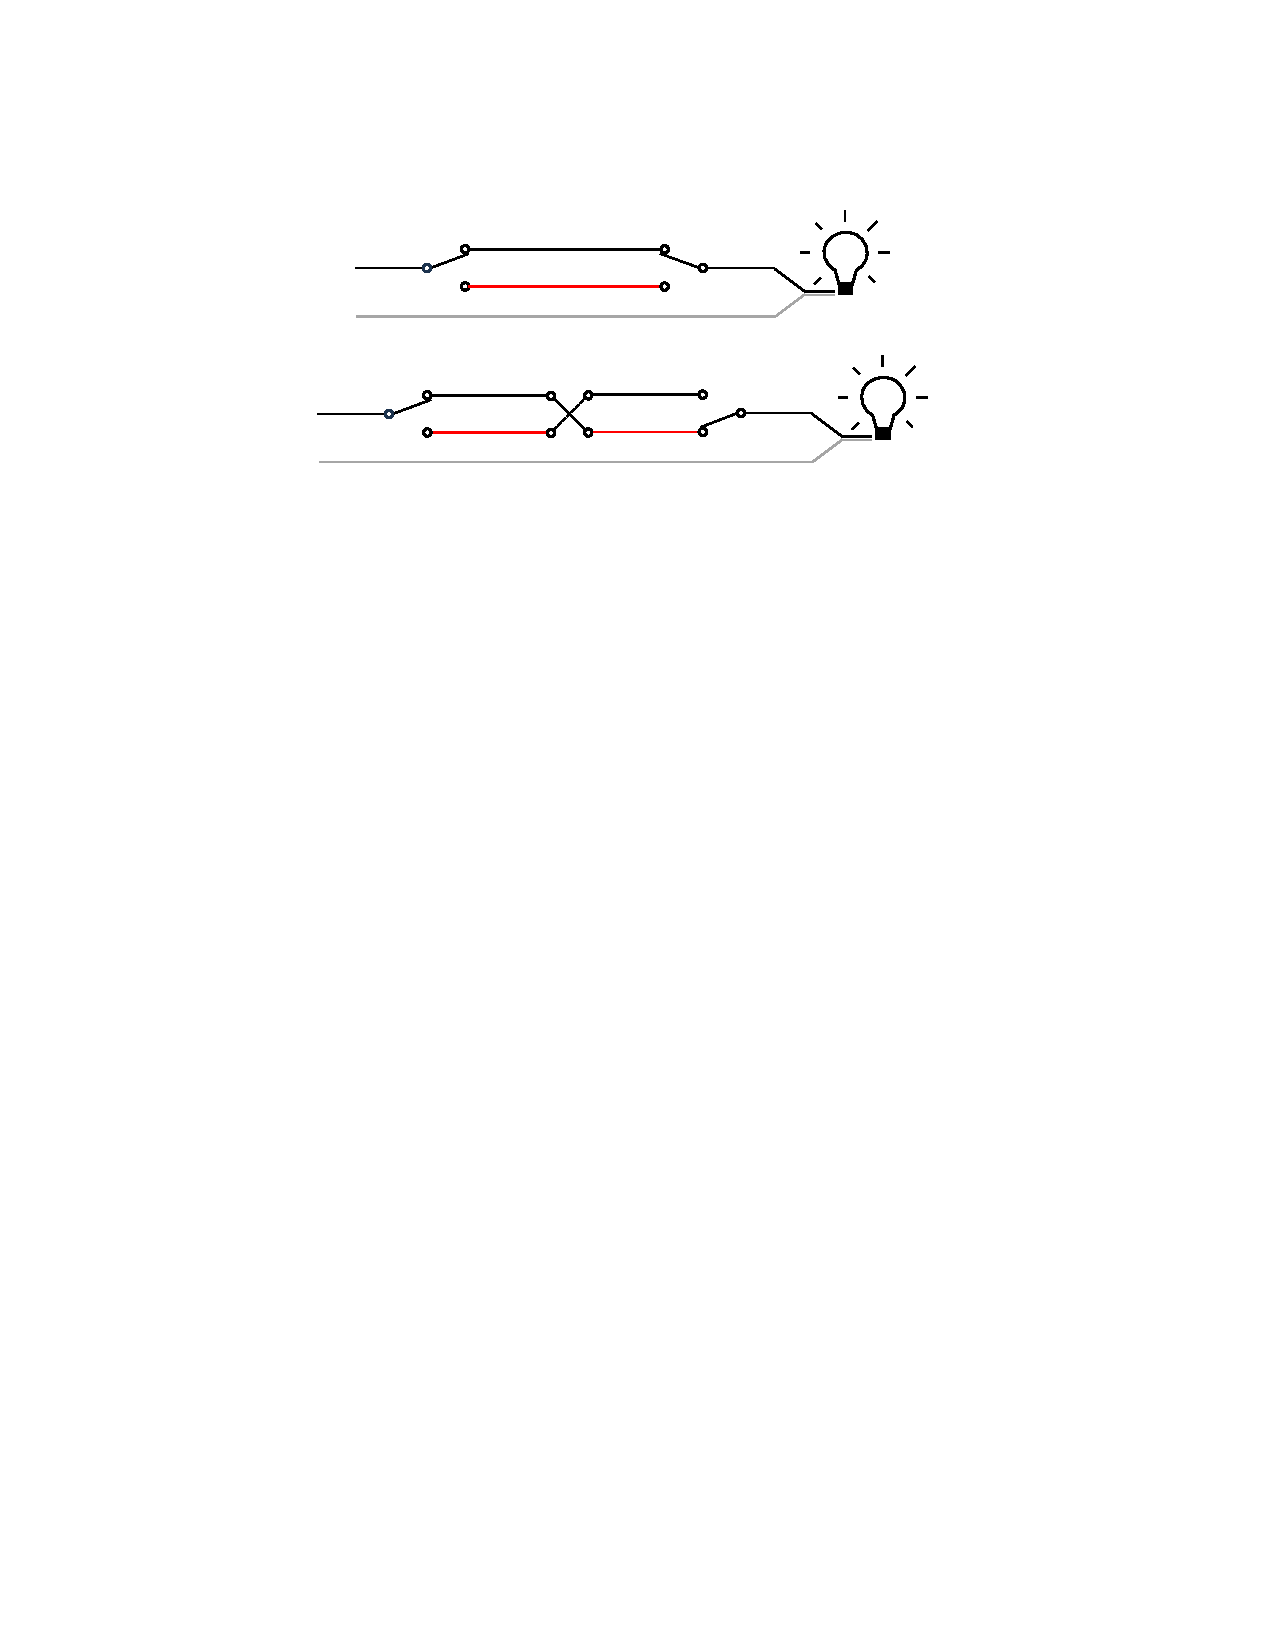
\includegraphics{appendices/switches/three_way_four_way.pdf}
\end{center}
Some switches are spring-loaded to automatically return to a particular state---called their \textit{normal} state---when they are not being actively held in place by someone's finger or by some other force.  For the SPST pushbutton switches below, different symbols are used depending on whether the switch is normally open (\textit{off} when not pressed), or normally closed (\textit{on} when not pressed).  In the case of an SPDT switch, the common terminal is always connected to \textit{one} of the two throws. The throw that is connected when not being pressed or activated is called normally closed (N.C.), and the throw that isn't connected is called normally open (N.O.).  
\begin{center}
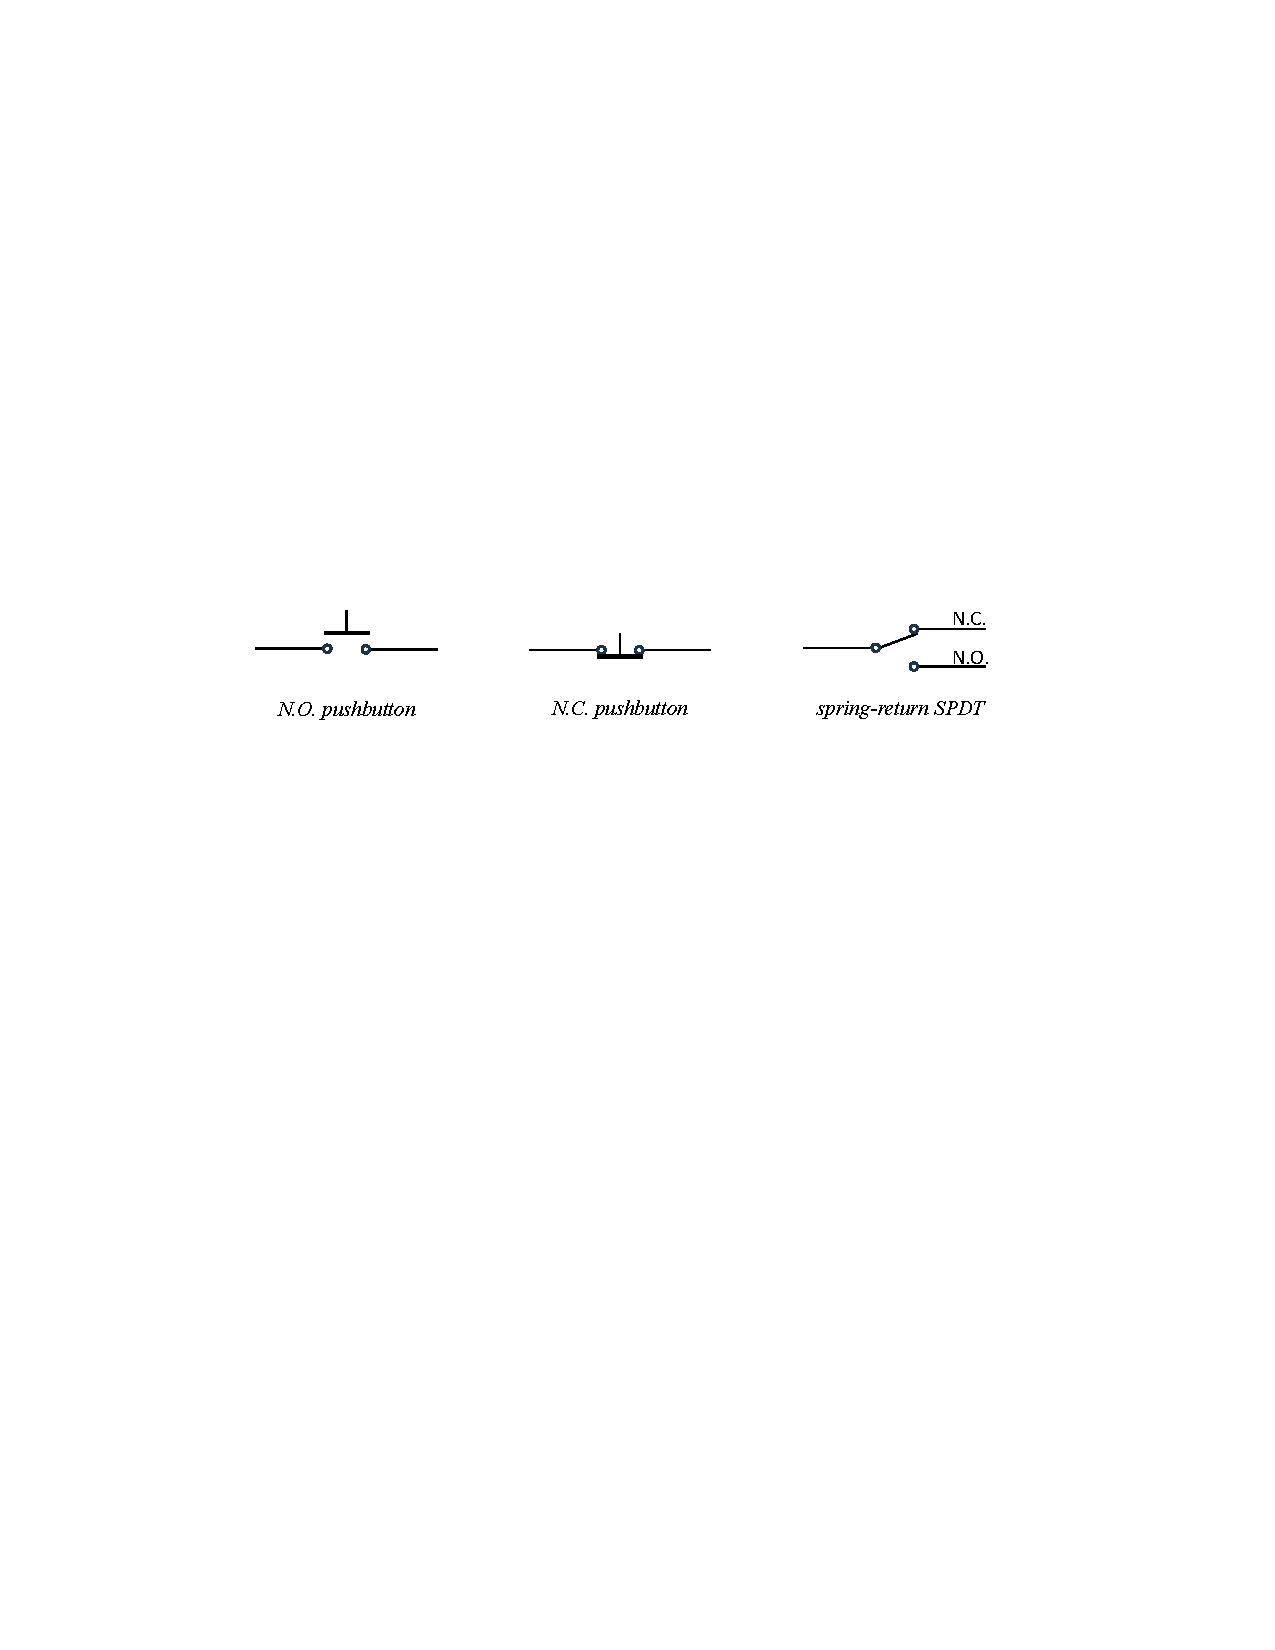
\includegraphics{appendices/switches/NO_and_NC.pdf}
\end{center}
